\chapter{Revisión de la literatura}

En este capítulo se realizará una revisión de los estudios y propuestas más innovadoras relacionadas con los algoritmos socioinspirados. Se tendrá en cuenta hasta dónde han llegado aquellos algoritmos en los que se basaron, los bioinspirados, qué impacto tienen en el panorama actual y de dónde surgieron los algoritmos socioinspirados. Además, se realizará un análisis general de aquellos algoritmos socioinspirados que resulten interesantes y se verá cómo de efectivos han resultado en problemas reales hasta la fecha.

\section{Estado del arte: algoritmos bioinspirados}

La algorítmica experimentó un antes y un después con la llegada de los algoritmos bioinspirados. El planteamiento tan visual a la par que efectivo que poseen dichos algoritmos incitó que poco a poco cada vez más investigadores se dedicasen a este campo. En particular, ha tenido especial éxito en la computación evolutiva, donde las propuestas más conocidas como los algoritmos de colonias de hormigas o de colmenas de abejas han resultado no sólo innovadoras sino también efectivas.

Los algoritmos \textbf{Ant Colony Optimization (ACO)}, los basados en los comportamientos de las colonias de hormigas, han sido los pioneros en este campo. Marco Dorigo fue el padre de los ACO, publicando en su tesis doctoral \cite{dorigo-thesis} en 1992 lo que él definió como <<Ant systems>>. A partir de esta primera aproximación, Dorigo continuó su investigación en dicha técnica, y años más tarde, en 1999, publicó su primera propuesta de algoritmo, explicando, en términos del autor, lo que él propuso como <<Ant algorithms>> \cite{ant-algorithms-dorigo}.

Además de la vertiente computacional, algunas de las primeras propuestas bioinspiradas también trataban de aplicar estas técnicas al hardware, en particular a mejorar el diseño de los sistemas. Sánchez et al. (1997) plantearon la investigación en este campo. En el 1st International Conference on Evolvable Systems, acontecido en Tsukuba, Japón, en 1996, presentaron en su paper \textit{Phylogeny, ontogeny, and epigenesis: Three sources of biological inspiration for softening hardware} \cite{bioinspired-systems-paper} las bases de la investigación en técnicas bioinspiradas, en este caso para dotar a sistemas hardware de procesos evolutivos. Más adelante lo publicaron en la revista IEEE Xplore \cite{bioinspired-systems-article}.

Estos ejemplos citados no son, sin embargo, nada más que la pequeña primera muesca en la historia de las técnicas bioinspiradas. Consultando una base de datos bibliográfica se puede observar un creciente aumento en cuanto a las publicaciones relacionadas con algoritmos bioinspirados. En la base de datos de SCOPUS estos datos pueden ser plasmados en una gráfica como la que se muestra a continuación.

\begin{figure}[h]
	\centering
	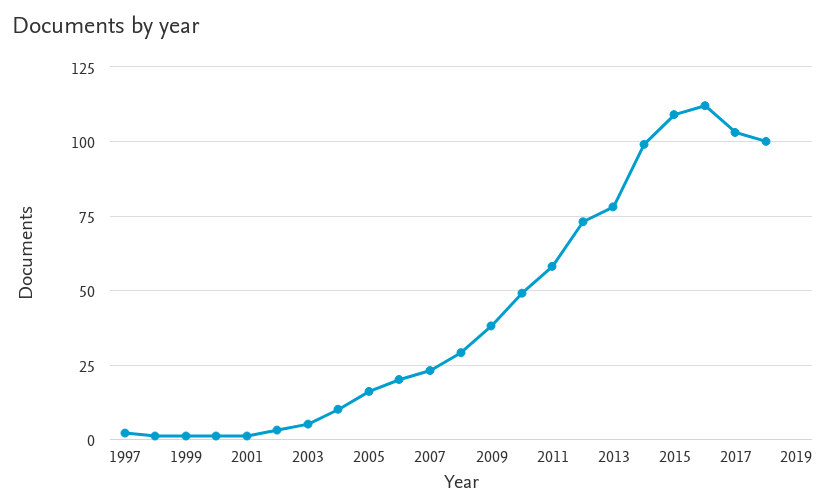
\includegraphics[scale=0.4]{imagenes/scopus-grafico-bioinspirados.png}
	\caption{Gráfico de publicaciones sobre algoritmos bioinspirados registradas en SCOPUS \cite{scopus-bioinspired}.}
	\label{grafica-scopus}
\end{figure}

Dicha gráfica refleja perfectamente el auge de los algoritmos bioinspirados; de menos de diez publicaciones por año hasta el año 2004 aproximadamente, hasta los más de 100 que llevan registrándose desde 2015. El éxito de estos algoritmos se fundamenta en dos pilares: su carga conceptual es sencilla de abstraer para cualquier usuario, y generalmente aportan buenos resultados a los problemas a los que se han enfrentado.

La principal motivación para construir algoritmos bioinspirados es simple, a la par que consistente: si un ser vivo ha evolucionado durante siglos y siglos hasta llegar a desarrollar una técnica con la que sobrevivir en la naturaleza, dicha técnica debe ser suficientemente óptima como para resultar digna de un estudio. Es por ello que se han propuesto multitud de técnicas que simulan el comportamiento de numerosos seres vivos en su búsqueda de un objetivo.

Actualmente existen algoritmos bioinspirados en cualquier rama del reino animal. Algoritmos de manadas de lobos o grupos de tiburones que acorralan a su presa, basados en bancos de peces que se mueven en grupo hacia una zona óptima, o incluso que simulan el movimiento de una polilla cuando se dirige hacia un foco de luz. Por supuesto, en los años de la explosión de los algoritmos bioinspirados (acorde con la gráfica de la figura \ref{grafica-scopus}, se podría considerar a partir de 2005), con tanta diversidad en las propuestas no tardaron en surgir técnicas cuyo concepto se basaba en un animal muy particular: el ser humano.

\section{Estado del arte: algoritmos socioinspirados}

Conocemos como \textbf{algoritmos socioinspirados} a aquellos que inspiran su funcionamiento en comportamientos basados en la especie humana, y que pueden aplicarse a resolver problemas de cualquier índole. Similar a sus contrapartes bioinspiradas, las técnicas socioinspiradas tienen en el centro de su modelo conceptual a un miembro que forma parte de la naturaleza, en este caso el ser humano, y se aprovechan de sus relaciones, formas de actuar y estilo de vida para intentar dar una solución óptima a un problema.

En el apartado anterior se defendía la investigación de técnicas bioinspiradas por la constante evolución en busca de supervivencia de las distintas especies animales, y esto sucede de forma análoga con las técnicas socioinspiradas. En el caso de estas últimas, sin embargo, la mejora de soluciones no se basa en la evolución genética de la especie a lo largo de los siglos y en la selección natural, sino en el desarrollo de técnicas que permiten a nuestra sociedad alcanzar metas colectivas o individuales. Dichas técnicas pueden resultar cotidianas, pero deteniéndose a analizar cada una de ellas se puede observar que dicho comportamiento se puede trasladar a un algoritmo que explore en un espacio de búsqueda.

Dada la multitud de variedades bioinspiradas que se han propuesto y estudiado desde el surgimiento de dichos algoritmos, era de esperar que se empezasen a valorar técnicas humanas para optimización de funciones. En el día a día de un ser humano suceden cuantiosas situaciones que, sin ser puramente consciente, le obligan a buscar una solución óptima a un problema menor, tales como buscar la ruta más óptima para desplazarse al lugar de trabajo, estimar la máxima cantidad de días que se puede pasar sin realizar la compra o en qué horas debe conectar un electrodoméstico para aprovechar al máximo el consumo energético. Son problemas en los que encontrar soluciones a corto plazo puede resultar trivial, pero las técnicas abordadas en este estudio abarcan temas más complejos, o a mayor escala.

Cabe destacar que son unas técnicas muy recientes, y que a día de hoy ni siquiera existe un estudio formal que analice algunas de las propuestas con experimentos y análisis de rendimiento, como se busca hacer en este Trabajo de Fin de Grado. De hecho, en la actualidad estos algoritmos se encuentran aún en una fase de divulgación y propagación, es decir, los investigadores priorizan buscar nuevas propuestas de algoritmos antes que analizar las ya existentes, bien por falta de ellas o por considerarlas poco prometedoras.

Kumar, Kulkarni y Satapathy \cite{socio-evolution-algorithm} han presentado la última propuesta socioinspirada actual, que data de abril de este mismo año, titulada \textit{Socio evolution \& learning optimization algorithm: A socio-inspired optimization methodology}. En este artículo, antes de explicar su algoritmo, los autores dan una pincelada sobre la situación de los algoritmos socioinspirados. En la gráfica ubicada a continuación se puede observar una clasificación de estos algoritmos, según los autores.

\begin{figure}[h]
	\centering
	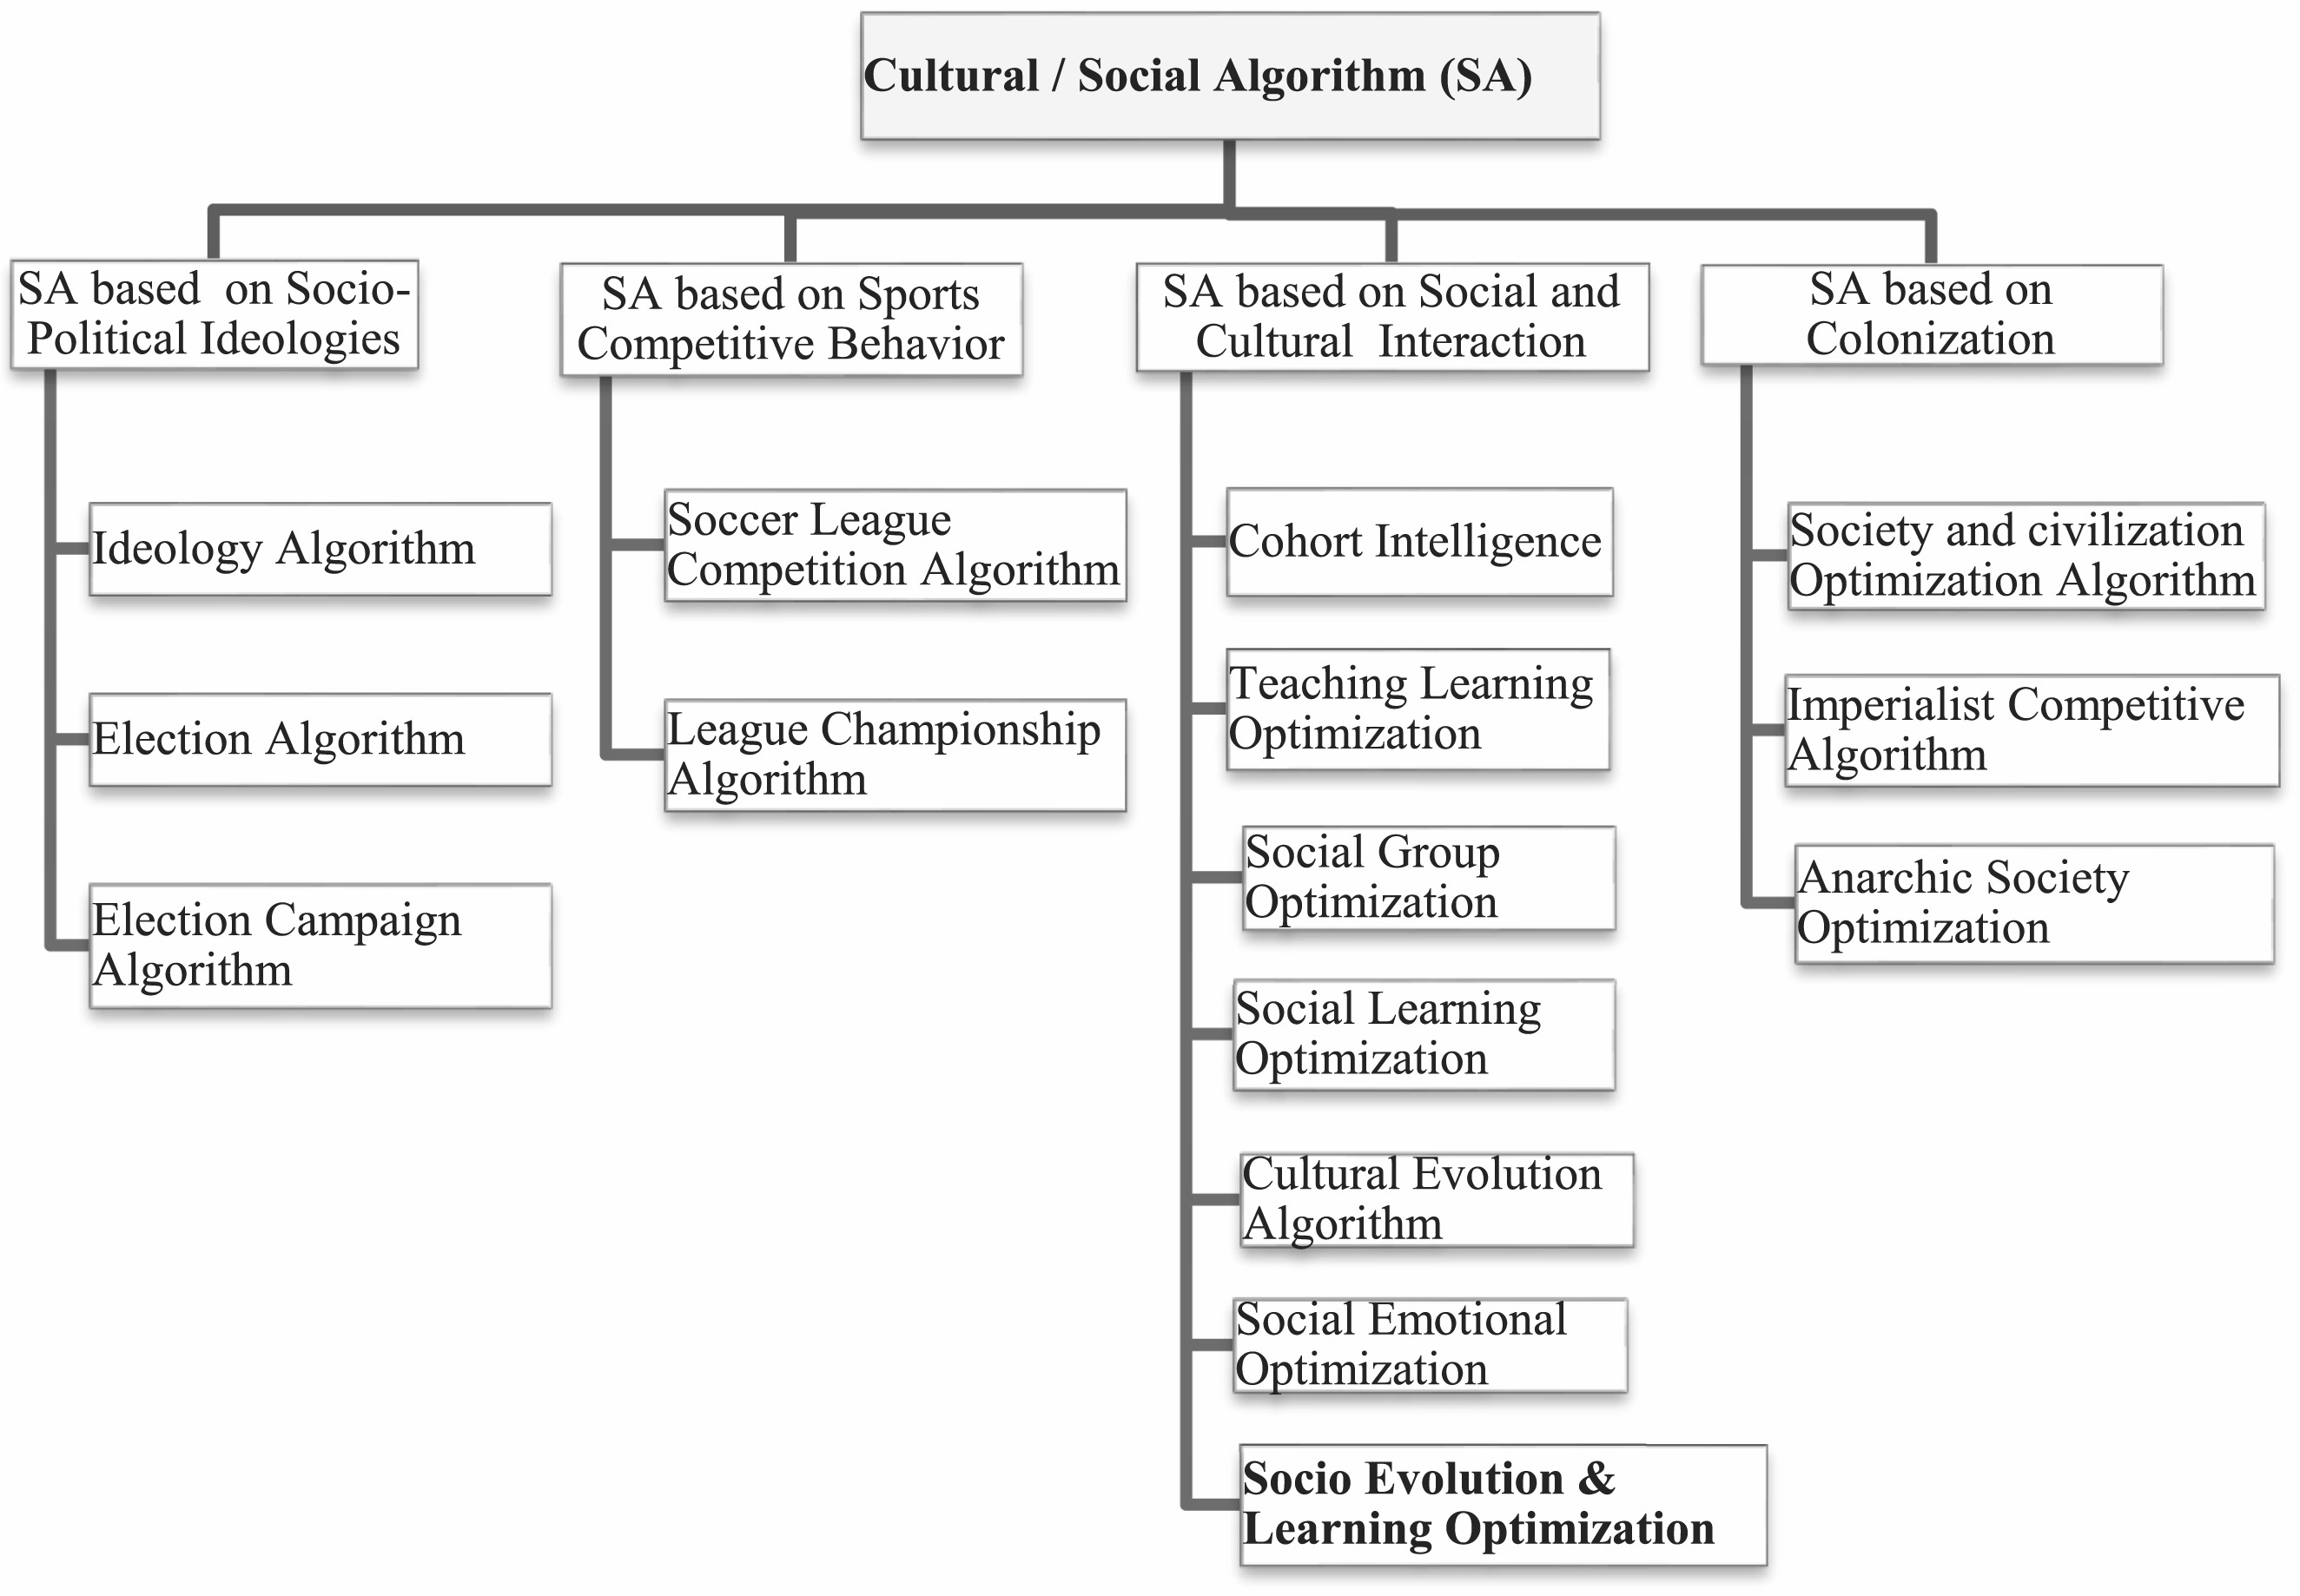
\includegraphics[scale=0.9]{imagenes/socioinspired-classification.jpg}
	\caption{Clasificación estimada de los algoritmos socioinspirados \cite{socio-evolution-algorithm}.}
	\label{clasificacion-socioinspirados}
\end{figure} 

En dicha gráfica se encuentran cinco de los seis algoritmos que son fruto de estudio de este trabajo: del grupo de socioinspirados basados en ideologías socio-políticas, el algoritmo \textit{Ideology Algorithm} (IA) \cite{ia-article}; del grupo de basados en competiciones deportivas, el algoritmo \textit{Soccer League Competition} (SLC) \cite{slc-article}; del grupo de basados en interacción social y cultural, el algoritmo \textit{Social Emotional Optimization Algorithm} (SEA) \cite{sea-chapter}; y del grupo de basados en colonización, los algoritmos \textit{Imperialist Competitive Algorithm} (ICA) \cite{ica-conference} y \textit{Anarchic Society Optimization} (ASO) \cite{aso-article} \cite{aso-chapter}.

El algoritmo restante, que no se muestra en esta gráfica, es \textit{Parliamentary Optimization Algorithm} (POA) \cite{poa-article}, y de haberlo incluido los autores en esta clasificación seguro que estaría en el primer grupo, los basados en ideologías socio-políticas. Su ausencia en la gráfica probablemente se deba al desconocimiento de su existencia por parte de los autores, ya que no es una clasificación muy extensa en la que haya habido necesidad de eliminar información.

Precisamente llama la atención la falta de propuestas en dicha gráfica. Los algoritmos socioinspirados están pasando por la primera etapa de la que se ha hablado en la sección anterior de algoritmos bioinspirados. Las propuestas son innovadoras, llaman la atención, pero pocos investigadores abandonan su campo de trabajo para volcarse con ellas. Poco a poco, si los resultados acompañan, irán desarrollándose nuevas técnicas que, retroalimentándose unas a otras, conseguirán dar consistencia a esta rama de la computación evolutiva.

En palabras de Kumar et al. \cite{socio-evolution-algorithm}, <<estos métodos han ganado popularidad por sus pautas sencillas para buscar soluciones óptimas en problemas computacionales reales y complejos>>. Como se había anticipado en la introducción, esta es la principal motivación para trabajar con algoritmos socioinspirados. Cuando se trata de aproximar a usuarios primerizos a la computación evolutiva, el primer escalón puede ser difícil de sobrepasar. Estos algoritmos aportan una visión más cotidiana, una forma de hacer comprender a casi cualquier persona cómo se puede explorar un espacio de soluciones sin tener que comprender a fondo el contexto de un algoritmo común de estas características.

Hablar de <<población>> en un algoritmo evolutivo no debe suponer ningún problema de comprensión para un investigador dedicado a este campo. Pero resulta mucho más atractivo si a esta población se le da un nombre propio, si se la asocia con un conjunto de individuos que una persona es capaz de reconocer y ubicar. Por ejemplo, con un parlamento político, o con los jugadores de una liga deportiva. Son sólo algunos de los casos que se plantean en los algoritmos estudiados en este trabajo.

Ya que una de las máximas de estos algoritmos es mantener la sencillez y hacer que las técnicas utilizadas sean lo más intuitivas posibles, la metodología que siguen para llegar a una solución óptima también debe ser asociable a conductas reconocibles. Al igual que las poblaciones están compuestas de soluciones habitualmente representadas como <<seres humanos>>, las técnicas evolutivas se corresponden a aquellas acciones realizadas por los mismos para llegar hasta su objetivo. Continuando el símil anterior, realizar debates políticos o jugar partidos de una temporada serían los ejemplos equivalentes.

Dentro de esta metodología siempre hay alguna figura o grupo que sobresale entre la población, y que constituye (o en caso de ser un grupo, contiene) al mejor <<individuo>>. Este se equivaldrá a la mejor solución encontrada para el problema, y es fácilmente reconocible si uno se abstrae a la capa socioinspirada del mismo. El mejor individuo de un parlamento político sería la figura del presidente, o el de una liga deportiva sería el mejor jugador admirado por todo el mundo.

Como se ha podido comprobar, el análisis funcional de los algoritmos socioinspirados es, a diferencia de lo que ocurre con otros algoritmos evolutivos de propósito general, bastante sencillo e intuitivo de transmitir. Esto es claramente debido a la naturalidad con la que un usuario puede asociar dichas pautas a acciones observables en su día a día. No obstante, la eficacia real de estos algoritmos, fuera de las funciones probadas en sus respectivos \textit{papers} o artículos, está aún por probar, ya que de momento no son partícipes de las grandes competiciones acontecidas en congresos, entre las que destacan las del Congress of Evolutionary Computation (CEC).

Sin embargo, sí que se han propuesto en distintas publicaciones algunas aplicaciones de estos algoritmos a resolución de problemas reales muy particulares. En el caso de aquellos algoritmos que se han estudiado en este trabajo, existe una aproximación del algoritmo \textit{Soccer League Competition} para optimizar el diseño de redes de distribución de agua \cite{slc-article}, u otra del algoritmo \textit{Anarchic Society Optimization} para manejar el controlador PID (\textit{proportional–integral–derivative}) de un Regulador de Voltaje Automático (\textit{Automatic Voltage Regulator} o AVR, en inglés) \cite{aso-article}.

Con el paso de los años es de esperar que estos algoritmos sean perfeccionados, sigan evolucionando y se utilicen cada vez en más problemas reales, al igual que sucedió en su momento con los algoritmos bioinspirados.
